\documentclass[conference,final]{IEEEtran}

\usepackage{graphicx}
\usepackage{epsfig}
\usepackage{subfigure}
\usepackage[hypertex]{hyperref}
\usepackage{subfigure}  
\usepackage{color}
\usepackage{srcltx}
% \usepackage{draftcopy}

\usepackage[small,it]{caption}

\usepackage{multirow}
\usepackage{ifpdf}

% \newcommand{\jha}[1]{\textcolor{red}{\bf Jha:} }
% \newcommand{\hartmut}[1]{\textcolor{blue}{\bf Hartmut} }
% \newcommand{\andre}[1]{\textcolor{green}{\bf andre} }
% \newcommand{\ole}[1]{\textcolor{red}{\bf Ole} }
% \newcommand{\everyone}[1]{\textcolor{red}{\bf EveryOne} }

\newcommand{\I}{\textit}
\newcommand{\B}{\textbf}
\newcommand{\T}{\texttt}

\newcommand{\upup}{\vspace*{-1em}}
\newcommand{\up}{\vspace*{-0.5em}}

\newcommand{\jha}[0]{}
\newcommand{\hartmut}[0]{}
\newcommand{\andre}[0]{}
\newcommand{\ole}[0]{}
\newcommand{\everyone}[0]{}

\newcommand{\fixme}[1]{ { \bf{ ***FIXME: #1 }} }
\newcommand{\jhanote}[1]{ {\textcolor{red} { ***Jha: #1 }}}
%\newcommand{\jhanote}[0]{}
\newcommand{\amnote}[1]{ {\textcolor{green} { ***AM: #1 }}}
%\newcommand{\amnote}[0]{}
\newcommand{\hknote}[1]{ {\textcolor{blue} { ***HK: #1 }}}
%\newcommand{\hknote}[0]{}
\newcommand{\jitter}[1]{{$\sigma(\alpha)$}}

\newif\ifpdf
\ifx\pdfoutput\undefined
  \pdffalse
\else
  \ifnum\pdfoutput=1
    \pdftrue
  \else
    \pdffalse
  \fi
\fi

\ifpdf
\DeclareGraphicsExtensions{.pdf, .jpg}
\else
\DeclareGraphicsExtensions{.eps, .ps}
\fi

\newenvironment{shortlist}{
  \begin{itemize}
  \setlength{\itemsep}{-0.1em}
}{
  \end{itemize}
}

\begin{document}


\title{\LARGE Grid Interoperability at the Application Level Using
  SAGA}

\author{\authorblockN{Shantenu Jha\authorrefmark{1}\authorrefmark{2},
    Hartmut Kaiser~\authorrefmark{1}, Andre Merzky\authorrefmark{3},
    Ole Weidner\authorrefmark{1}} \authorblockA{\authorrefmark{1}
    Center for Computation and Technology, Louisiana State University,
    Baton Rouge, Louisiana, USA, 70803}
  \authorblockA{\authorrefmark{2} Department of Computer Science,
    Louisiana State University, Baton Rouge, Louisiana, USA, 70803}
  \authorblockA{\authorrefmark{3} Vrije University, Amsterdam,
    Netherlands} }

% \author{\authorblockN{AnyBody\authorrefmark{1},
%      EveryBody\authorrefmark{1}, NoBody\authorrefmark{1},
%      SomeBody\authorrefmark{1}}}

\maketitle

\begin{abstract}\jha
  SAGA is a high-level programming abstraction, which significantly
  facilitates the development and deployment of Grid-aware
  applications. The primary aim of this paper is to discuss how each
  of the three main components of the SAGA landscape -- interface
  specification, specific implementation and the different adaptors
  for middleware distribution -- facilitate application-level
  interoperability. We discuss SAGA in relation to the ongoing GIN
  Community Group efforts and show the consistency of the SAGA
  approach with the GIN Group efforts.  We demonstrate how
  interoperability can be enabled by the use of SAGA, by discussing
  two simple, yet meaningful applications: in the first, SAGA enables
  applications to utilize interoperability and in the second example
  SAGA adaptors provide the basis for interoperability.
%   Ginpaper~\cite{gin_paper} by Reidel, discusses applications that are
%   not truly interoperation across grids. they are what we call
%   grid-unaware applications. saga enables grid aware applications to
%   establish interoperability.  Saga merges the distinction between
%   interoperation and interoperability.
%   Explain why these are grid-applications that require
%   interoperability -- which then is not just a nice talking point, but
%   a necessary feature.
%   Interoperation is not sufficient; interoperability is necessary.
\end{abstract}

\begin{keywords}
  eScience Application, Application, Inter-operation, Distributed
  Infrastructure Deployment, Distributed Application Programming,
  Cactus, SAGA,
\end{keywords}

\section{Introduction}% \textcolor{blue}{Jha}}

Attempts to make the Grid -- a global computational infrastructure a
reality~\cite{foxbook}, have been ongoing for some time.  While there
exist islands of infrastructure that can be successfully marshaled for
a task, the fundamental idea that inspired the ``Grid'' analogy --
indistinguishable computational resources and seamless sharing
of resources across administrative, technical and distributed domains
is not reality yet.
% idea or the original metaphor that inspired the term ``Grid
% Computing'' which was predicated on

%unfortunately are not there yet. There

A lot of effort has been invested in trying to connect these
islands\footnote{We consider the following -- Grid-of-Grids, Federated
  Grids and Inter-Grids -- to be equivalent and representative of the
  situation when resources from two or more distinct Grids are
  utilized.  Distinct Grids are those which differ either at the
  administrative, middleware or service \& policy level}. In
particular the pioneering efforts of the GIN Community
Group\cite{gin_url} at the OGF~\cite{ogf_url} at identifying and
solving the problems related to interoperation are laudable. On the
other hand, there have been impressive application-centric efforts to
interoperate across distinct Grids, as illustrated in References
\cite{Cactus_GordonBell, clade06} - to name just a few~\footnote{The
  conference series - Challenges of Large Scale Applications in
  Distributed Environments, provides an interesting sample of
  application-centric efforts at utilizing federated Grids}.  These
attempts at providing interoperation -- that is quick, workable
solutions -- represent two different approaches to the problem.  In
the first approach (symbolized by the GIN group efforts), the focus
has been on attempting to provide the basic {\it services} that are
required for Grids to interoperate; approaches symbolized by the
application groups have been aimed at enabling specific applications
to utilize federated Grids.  The successful interoperation of Grids in
the latter case, is thus specific to the application(s) under
consideration, i.e., what might represent interoperation for one
application might not represent interoperation for a different
application.  GIN efforts can be viewed as a bottom-up approach,
whilst application-centric efforts as top-down.  So far all attempts
-- whether aimed at providing interoperation at the service-level or
application-level -- have been quick and short term solutions, in
order to begin utilizing Grid resources, for it is not practical, nor
desirable that applications wait for federated resources to get every
last detail and requirement in place.

e-Science applications must be able to utilize e-Infrastructure --
whether sophisticated services, or the next generation networks or
customized supercomputers -- to perform better, faster and different
domain specific research~\cite{hey04, hey05}.  The question is how can
we design and develop e-Science applications, that on the one hand are
not limited by the heterogeneity of infrastructure that exists at any
given point in time, while on the other hand being immune to the
evolving nature of such infrastructure?  In other words, how can we
compose applications so as to not depend on the underlying
infrastructure -- either in a dynamical sense (i.e., over a period of
time), or different infrastructure at essentially the same time.  

We contest that there exists at least one approach that address both:
design applications using widely supported, standardized high-level
interfaces. It is reasonable to posit that a necessary requirement for
applications to work over federated Grids is to abstract out the
non-essential details of the specific Grids and one way of effectively
doing this is through the use of such standardized, application-level
interfaces. Specifically, we suggest that SAGA~\cite{saga_web} - which
provides simple method calls at the right level of abstraction for the
most commonly required Grid-functionality provides most of the
application requirements for interoperability. 

% Irrespective of the scalability of the solution, or the time-scale
% over which the solution is attempted or required, 
% We will argue in the next section that the need for seamlessly
% utilizing federated Grids is critical.

\noindent We follow the working-definitions of interoperation and
interoperability as provided by the GIN group~\cite{gin_url} and
Reference~\cite{gin_paper}.  We extend them to include application
level interoperation or interoperability, which to a first
approximation, can be thought of as the ability of applications that
require explicit Grid functionality to be able to utilize resources
across federated Grids. The primary aim of this paper is to discuss
and highlight SAGA as a critical enabling technology for such
application-level interoperability (ALI). In principle, any
sufficiently high-level programming interface with widespread support
and commitment to being supported can be used in lieu of SAGA; it just
happens to be the case that no such similarly broadly usable interface
exist\footnote{If, for example, OGSA would provide an application level
interface to OGSA services, which would in fact be supported by the 
majority of Grid middlewares, there would be no need for an API such as 
SAGA.}!
In section 4, in addition to SAGA enabling interoperability
both in principle and in practise, we will discuss how the specific
details of our implementation enhance the ability to interoperate
across federated Grids.

% Standardization should not be over emphasized but it is critical.
% Note it is also stated as the major advantage of OGSA-BES and JSDL in
% the ginpaper~\cite{gin_paper}

\noindent This paper is structured as follows: In the next section we
elaborate further what we refer to as Application-level
interoperability (ALI), and distinguish it from service level
interoperability/interoperation (SLI).  Section~\ref{sec:saga}
presents the motivation and the basic design principles behind the
specification of a high-level programming abstraction such as SAGA;
this section also sketches the main packages that are currently
specified and implemented. An interesting and pedagogically important
part of Section~\ref{sec:saga} is a discussion of how SAGA relates to
the five current areas of GIN activity.  Section~\ref{sec:saga_imp}
discusses how good software design principles have been employed in
the (first) implementation of the SAGA specification and how it
supports application-level interoperability across distinct middleware
distributions.  Section~\ref{sec:app} discusses a couple of simple,
yet interesting applications that we have developed using SAGA, that
not only \I{require}, but also \I{implement} application-level
interoperability.  We conclude with a discussion and analysis of our
work and some implications for the future of interoperability.

\section{Application level interoperability}\label{sec:ALI}
% \textcolor{blue}{Jha} } 

In this section we will elaborate further on what we mean by
application level interoperability, but before that it is important to
clarify the type of applications in the scope of this paper.  Using a
high-level taxonomy, we can classify\footnote{The aim is not to
  provide rigorous definition, but a classification scheme.}
applications as either Grid-aware or Grid-unaware.  Any application
can to a first approximation, be thought of as a Grid-aware
application if it is cognizant of the underlying distributed
infrastructure, and/or for which there is a requirement to explicitly
exploit, run or utilize the distributed infrastructure.  Simple
examples of Grid-aware applications are the class of tightly coupled
MPI jobs -- which are generalizations of parallel applications to
parallelized and distributed applications.  For example, MPICH-G2
applications require cognizance of the distributed resources in their
RSL description.  Additionally, there are ``first principles'' Grid
applications, such as GridSAT~\cite{gridsat03} and applications which
based upon resource aware ``learning'' algorithms~\cite{
  majority_voting}, which need to explicitly marshal distributed
resources. For these applications the resource utilization is often
dynamic and unpredictable; interestingly, the resource requirements
and utilization might possibly be dependent upon both the execution
trajectory and underlying infrastructure.

\begin{figure}
\begin{center}

\includegraphics[scale=0.6]{../diagrams/application_scope}
\end{center}
\caption{A high level classification of applications into Grid aware
  versus Grid unaware. Most Grid-unaware applications can make do with
  service-level interoperation.This diagram also illustrates the
  typical mechanisms (and differences) in how Grid-aware and
  Grid-unaware applications access the service and resource layer. \upup}
\label{fig:scope}
\end{figure}

Grid-unaware applications, are those that are not cognizant of the
environment that they are executed in, and their behavior, resource
requirement and possible execution trajectory is {\it independent} of
the resources.  Examples include sandboxed applications developed
using say BOINC infrastructure, or an application launched in a portal
or using a meta-scheduler such as GridWay.
%Are examples of grid-unaware applications.  
Both portals and meta-schedulers qualify as Grid-enabled Programming
Environments as shown in Fig.\ref{fig:scope}.

\noindent Some defining features of ALI include:
\begin{enumerate}
\item Other than compiling on a different or new platform, there are no
  further changes required of the application
\item Automated, scalable and extensible solution to use new resources,
  and not via  bilateral or customized arrangements
\item Semantics of any services that an application depends upon are
  consistent and similar, e.g., consistency of underlying error
  handling and catching and return
\end{enumerate}

For Grid-unaware applications, it should be easy to see why
applications that utilize distributed resources via portals, or by
sandboxing or through other Grid-enabled Programming Environments,
don't require ALI, but they do require SLI, such as the ability to
submit jobs and transfer files directly between middleware
distributions. Establishing interoperation/interoperability across
Grid-unaware applications is {\it relatively} easier than to do so for
Grid-aware applications.  Not surprisingly, interoperability is a
necessary condition for any successful Grid-aware application and thus
is the real challenge.  For the remainder of this paper, we will
discuss ALI with a focus on Grid-aware applications.  In addressing
the relationship between ALI and service-level
interoperability/interoperation (SLI), the issue is not that of
whether ALI and SLI are orthogonal problems, or if SLI is a necessary
condition for ALI, but how does one influence the other.  For example,
applications based upon the master-client programming model don't
really require SLI but do require ALI.  It might be obvious that ALI
would benefit from SLI, i.e., if SLI is available, ALI is easier to
implement, but the converse is not always true, or even intuitive.

%and discuss ALI with such applications in mind. For the rest of this paper, 
% is establishing interoperability (or even interoperation) for
% Grid-aware applications.

The first point almost necessarily implies the need for a high-level,
standardized API; as we will discuss such an API provides a necessary
condition for ALI, but by itself does not provide a sufficient
condition if not implemented or supported completely.  ALI can be
achieved in various ways: probably the simplest example of ALI comes
from the successful deployment of MPICH-G2 based applications, which
in turn requires simply extending the MPI library to an MPICH-G2
library where appropriate. Also as alluded to, high-level interfaces
that provide functionality beyond messaging are useful.  In addition
to the above three requirement, there exist features that would be
{\it nice to have}, as they would make interoperability more robust
and extensible. Such features include performance
estimates/guarantees, or service-level agreements (SLA) between
resource providing Grids.  For example, there are Grid-aware
applications for which, interoperability is predicated on the ability
to federate resources from distincts Grids synchronously, which in
turn requires features such co-scheduling, or at the very least a
Quality of Service (QoS) assurance or SLA that facilitate this.  In
such cases ALI requires consistency and agreements at the policy level
(going beyond firewalls); this is unlikely to be the case for SLI.
Not having these agreements will lead to adhoc arrangements, say over
the phone and system administrator exchanges, and which at best, can
lead to interoperation.  Such interoperation has been shown to work
for tightly-coupled applications such as NeKTAR and
Vortonics\cite{clade06}, but it is also realized that such solutions
are not scalable.

Finally and to state the obvious, for both Grid-aware and/or
Grid-unaware applications, there needs to be operating-system level
and middleware level support for whatever framework the application is
developed on. Revisiting the MPICH-G2 application for example, the
platform should not only provide a local implementation of MPI, but
also compatible Globus services; however, much of this requirement is
not specific to distributed computing hence we do not elaborate
further.

% \noindent what aspects of these are best implemented at the
%   middleware level? what aspects are best explicitly controlled by
%   user?  (this is a recurring theme by the way)

% \noindent for grid aware applications -- what grid components are
%   required, i.e.  distribution does not change with middleware and
%   interaction does not change or if they do they need to provide
%   intelligent support for this.

% \noindent lessons to be learnt from parallel programming history,
%   openMP and MPI (ie say a hybrid messaging system). list some of the
%   main issues that were faced by the integration, interoperation of
%   applications on these hybrid systems

% \noindent not enough that the same consistent set of  services shold
%   be provided, often just replicated -- that makes it trivial service level 
%   interoperability -- but that any one grid can work in tandem to solve
%   the problem even if different requirements might be
%   needed

% \noindent interoperation efforts so far have been aimed at
%   grid-unaware applications.


\section{SAGA}\label{sec:saga}
% \textcolor{red}{everyone}}

The Simple API for Grid Applications (SAGA) is an API standardization
effort within the Open Grid Forum (OGF)~\cite{ogf_web} -- an
international committee that coordinates the standardization of Grid
middleware and architectures. SAGA provides a simple, POSIX-style API
to the most common Grid functions at a sufficiently high-level of
abstraction so as to be able to be independent of the diverse and
dynamic Grid environments.  SAGA has been often been referred to as
the MPI~\cite{mpiforum_url} for Grid Programming, in that is a simple,
high-level programming abstraction that provides most of the
functionality. In addition to being simple, a noteworthy and critical
feature of SAGA is that it is on the road to becoming a community
standard, thus strengthening the analogy with MPI.  The interface
defined by the SAGA specification is grouped as a set of functional
packages, which we discuss in this section. Version
1.0~\cite{saga-core} of the specification has been submitted to the
OGF editorial pipeline and is currently under review.

\subsection{SAGA Packages:}%\textcolor{red}{Ole}}

The SAGA packages are as follows:

\begin{shortlist}
\item File package - provides methods for accessing local and remote
  filesystems, browsing directories, moving, copying, and deleting
  files, setting access permissions, as well as zero-copy reading and
  writing
\item Replica package - provides methods for replica management such
  as browsing logical filesystems, moving, copying, deleting logical
  entries, adding and removing physical files from a logical file
  entry, and search logical files based on attribute sets.
\item Job package - provides methods for describing, submitting,
  monitoring, and controlling local and remote jobs. Many parts of
  this package were derived from the largely adopted
  DRMAA~\cite{drmaa_url} specification.
\item Stream package - provides methods for authenticated local and
  remote socket connections with hooks to support authorization and
  encryption schemes.
\item RPC package - is an implementation of the GGF GridRPC
  API~\cite{gridrpc_url} definition and provides methods for unified
  remote procedure calls.
\end{shortlist}

The two critical aspects of SAGA are its simplicity of use and the
fact that it is well on the road to becoming a community standard.
Simplicity arises from being able to limit the scope to only the most
common and important grid-functionality required by applications.
There a major advantages arising from its simplicity and imminent
standardization.  Standardization represents the fact that the
interface is derived from a wide-range of applications using a
collaborative approach and the output of which is endorsed by the
broader community.

\subsection{SAGA In Relation to GIN:}

Having outlined SAGA, its features and design goals, we now discuss
its relationship to the (five) areas of GIN.

\subsubsection{SAGA and Information Services and Modeling}

The GIN effort for interoperation of various information services
focuses mainly on the identification of common information elements,
and of schema translators and data providers (adaptors) to access
these information elements.  That additional layer on top of the
individual middleware solution provides a GLUE based representation of
the individual information resources, via a BDII-based (i.e. LDAP
based) infrastructure.

SAGA on the other hand provides the application level access
mechanisms (API, storage management, query language) which allows
applications to easily access and use Grid resource and application
information.  SAGA exposes, however, only those information elements
which are of interest to the applications (i.e. does not expose
information which are \textit{internally} used for scheduling
decisions).  Additionally, SAGA allows the transparent management of
custom information items within the same framework, which enables
Grid-aware  applications to use the information service paradigm to
persistently store, search and retrieve application level information.
The resource level information used by GIN for SLI are thus extended
by application level information used for ALI.

\subsubsection{SAGA and Job Submission and Management}

% \jhanote{There is a very important need to have a full long paragraph
%   highlighing the connection between the saga job submission and
%   OGSA-BES.}

GIN, and indeed many recent and relevant Grid projects, rely on
OGSA-BES (OGSA Basic Execution Service) and JSDL (Job Submission and
Description Language) for interoperation of job submission and job
management.  BES and JSDL can indeed be used on a wide variety on Grid
middleware distribution, as both standards are intentionally easy to
map to other, existing job description languages and submission
systems.

The SAGA job management API exposes the same basic functionality as
BES, and provides additional program level simplifications and
abstractions to the application.  For example, the id of a submitted
job in SAGA, is represented as an object, so that actions on that job
can be performed directly, without the need to explicitly contact the
respective job service.

Incidentally, the job state model exposed by SAGA is exactly the same
as the job state model defined by BES.  This is not a coincidence, as
the state model was designed by the SAGA and BES groups at the OGF
together. Due to the two-level state-model, it can, (a)
accommodate all higher level states which SAGA calls and BES actions
can actually act upon, and (b) can represent all additional states any
specific job management system may internally use.

The SAGA Job description is represented by a subset of JSDL and
JSDL-SPMD keywords, and has some additional keywords which are used to
allow for application level job scheduling.  Even though JSDL is not
supported explicitly, the application level job descriptions are thus
easily mapped to JSDL documents, and the SAGA implementation can
transparently use the BES/JSDL layers to submit and manage the jobs.
For application level interoperation it is important to mention that
jobs created from within an application can be controlled,
communicated with, and reaped by that application: this allows for
extremely simple application level implementations of job cloning,
spawning, and task farming scenarios.  Also, SAGA allows easy
bootstrapping of distributed applications, as job IDs can easily be
exchanged over the information service interfaces mentioned before.

\subsubsection{SAGA Data Management and Movement}

% \jhanote{data movement seems to be easy; we have gridftp adaptors,
%   which seem to be the ``standard'' way of doing things; note
%   Ref.~\cite{gin_paper} complains about how when using different
%   protocols - such as http they have problems due to lack of
%   sufficient support! Explain how SAGA can - at least in principle -
%   take/handle ``any'' protocol}

% \jhanote{data management seems to be harder; explain how the ``SRB''
%   and ``SRM'' islands can be overcome (pg 5 of~\cite{gin_paper}), if at
%   all}

The GIN community identified~\cite{gin_paper} GridFTP~\cite{gridftp}
as \I{''lowest common denominator for data movement in Grids today''}.
Other, more advanced data movement infrastructures, such as various
Grid storage managers or replica systems, are assumed to form
\I{islands}, i.e. disconnected sets of resources which do not (easily)
allow the interchange of data sets.

The SAGA approach differs in that it completely hides the details and
differences of all data movement and data management infrastructures.
As an API, SAGA cannot really provide the interoperability the
infrastructure seem (according to GIN) to be inherently missing, but
can at least free the application programmer from the need to
differentiate at a programmatic level.  For example, SAGA allows to
specify the location of a file as
'\T{any://remote.host.net/dir/file.typ}'.  The pseudo-schema \T{any}
allows the SAGA implementation to automatically choose a suitable
schema, depending on the deployed middleware.  That mechanism cannot,
of course, guarantee that the file is indeed available via (literally)
any schema or protocol, or that the available schema provides the full
scope of access mechanisms defined by SAGA, but the application
programmer is nevertheless freed from the need to explicitly
switch the application code for each island.

\subsubsection{SAGA Authorization and Identity Management}
%\jhanote{just something brief; first three are important}

 \I{``Identity management and authorization of resource usage
 should, be performed transparently at the application level''} is a
 repeatedly stated end user requirement, and the SAGA API follows that
 guideline.  It exposes only minimal interfaces for identity
 management, and most authentication and authorization processes
 are not exposed at the application level.  That allows to
 interface a SAGA implementation to a wide variety of security
 approaches, including of course GIN-AUTH/GIN-VOMS services.

\subsubsection{SAGA and Cross-Grid Applications}
SAGA as an API cannot, by design, provide service level Grid
interoperability.  SAGA implementations can, however, very well
complement the GIN efforts at the application level, as they allow
applications to be \I{easily} written and to \I{seamlessly} utilize
the infrastructure.  With SAGA, the same application code can, (a)
run on multiple Grids, and (b) interoperate with applications running
on other Grids, thus allowing for truly interoperable Grid aware
applications..
% , if the SAGA implementation and the Grid middleware
% supports that interoperation -- as is the case for GIN environments,
% and our SAGA implementation.  This in turn allows for truly
% interoperable Grid aware applications.

\subsection{SAGA and ALI:}

\begin{figure}
\begin{center}
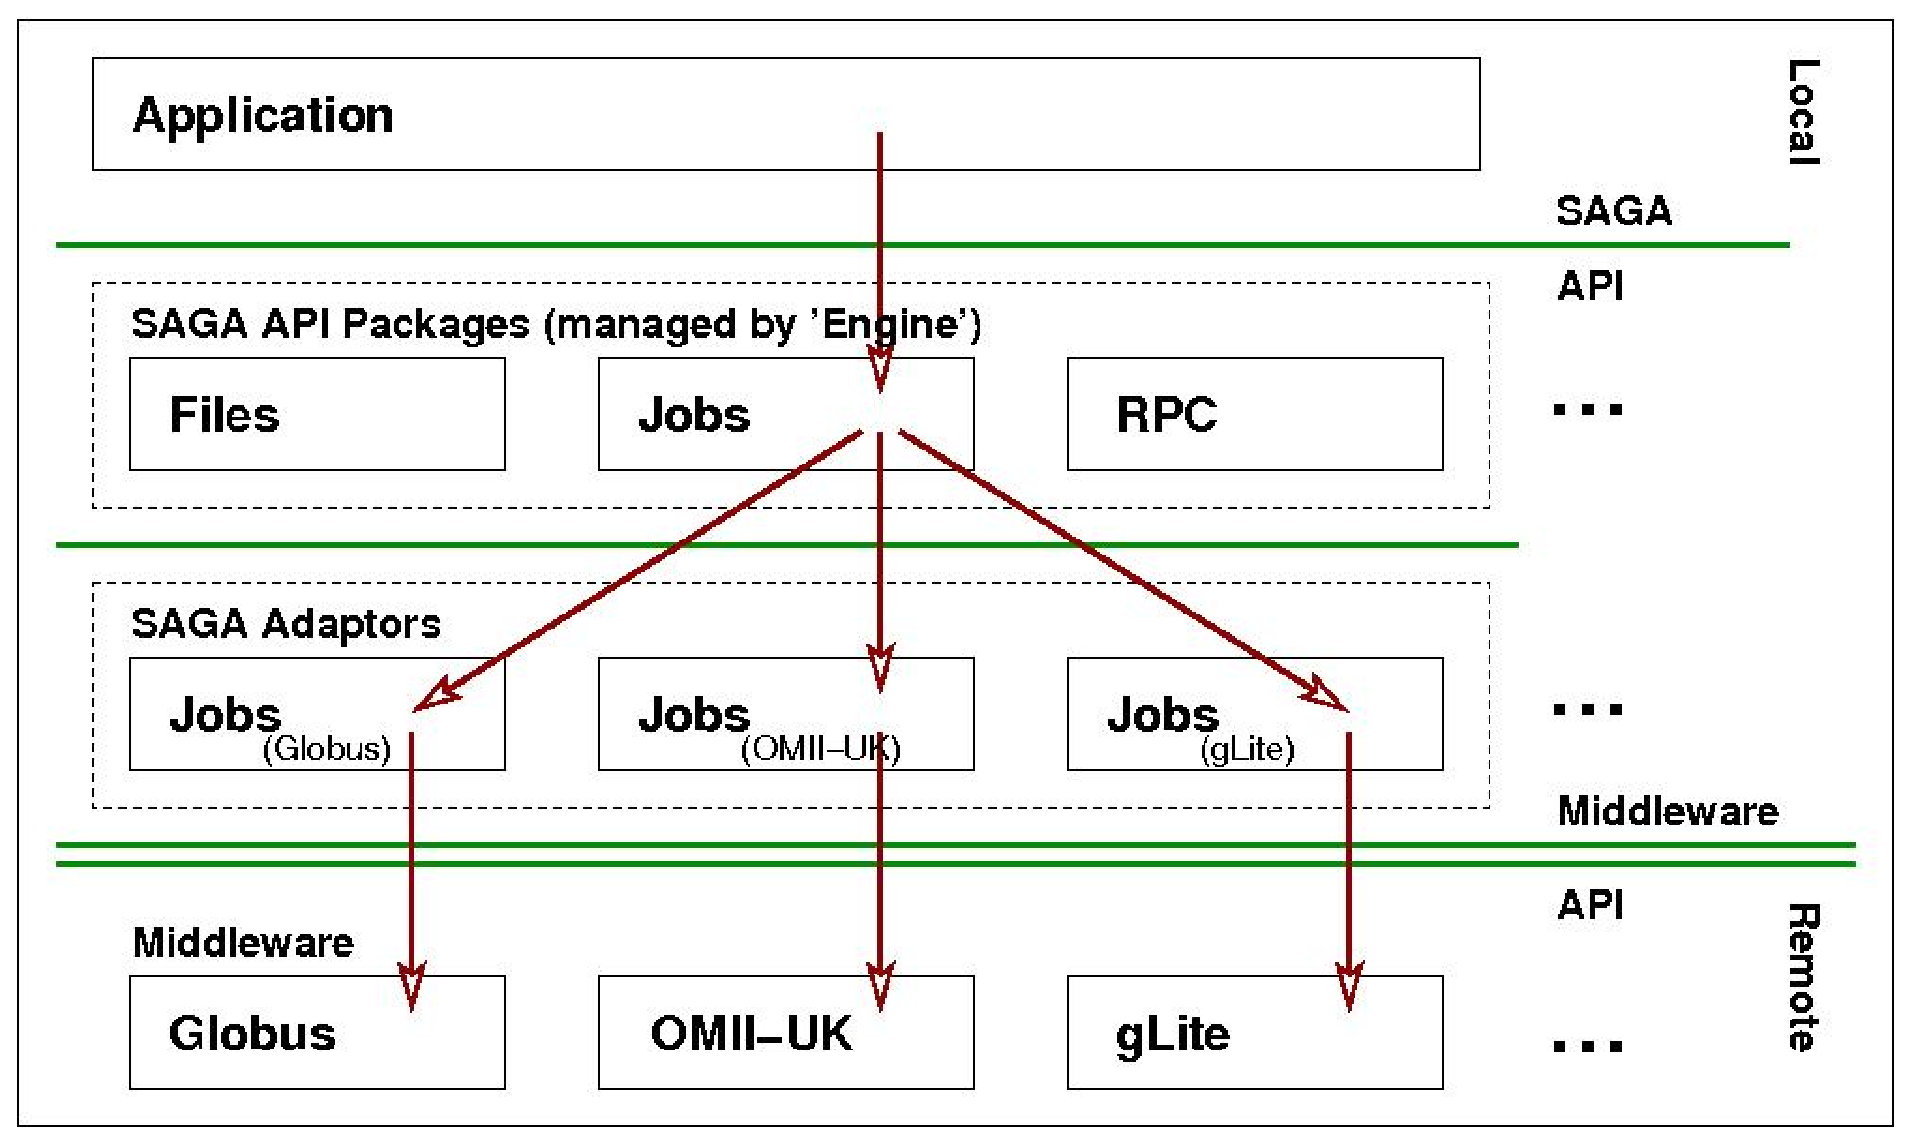
\includegraphics[scale=0.6]{../diagrams/saga_architecture}
\end{center}
\caption{An example of how SAGA is an effective mechanism for Grid
  Interoperability for job submission.\upup}
\label{fig:saga_arch}
\end{figure}

The previous section discussed how SAGA relates to the five areas of
GIN. In this brief section, using the example of job launching, we
will outline how SAGA provides ALI.  Figure~\ref{fig:saga_arch} shows
how the appropriate adaptors (i.e. middleware bindings) are invoked by
the SAGA engine in order to provide correct execution on different
Grid middleware distributions. The basic architecture and the
mechanism are the same for other (functional) packages (e.g. Files and
RPC). We will provide details in the next section about the design and
intelligence required for SAGA to implement this properly. But as
shown in Fig.~\ref{fig:saga_arch} the relevant point here is, SAGA
provides ALI by having the same function calls from within the
application but, with the appropriate execution and different
implementation within adaptors on varied middleware distributions.
Thus in addition to the implementation of the core engine, SAGA's
ability to provide ALI is as good as the adaptor set for the
middleware distribution that it aims to work on.  As each adaptor
usually is aimed at connecting to a specific middleware and all Grid
related API calls are dispatched by the adaptors to the appropriate
middleware functionality, the adaptor quality and their syntactic and
semantic uniformity with regard to the SAGA specification is of
central importance for ALI.

%\jhanote{Does someone want to clarify/elaborate here?}
%\hknote{I did, please check!}

% \jhanote{Note sure: ALI is both vertical and horizontal, SLI is mostly
%   horizontal. I think when taken from the application perpsective
%   there is nothing hortizontal; i.e., even if you want to issue a file
%   transfer command, it is coming from the application, thus the
%   appropriate adaptor is called. Is this a case of
%   another-level-of-indirection?}

% SLI interoperability on the other hand is about horizontal level
% control flow/interoperability, i.e. how to get Globus talking to
% UNICORE for example.  (i) Is it OK to say that ALI builds upon SLI? Or
% is it all in the SAGA adaptors? Need to clarify/elaborate (ii)

SAGA as it stands can provide most, but not all requirements for ALI
as outlined in Section~\ref{sec:ALI}. Specifically, it cannot provide
features such as QoS, co-scheduling and currently does not have
support for SLA.  We contest that this is not an intrinsic limitation
in the design of SAGA, but a design decision to ensure the ``S'' (for
simple) in SAGA as well as reflection of the complexity of solving
implementation details of co-scheduling across federated Grids.

% Additionally, it must provide the ``simple'' and ``easy-to-use'' API
% the SAGA standard is intended to specify.  While developing the SAGA
% implementation we

\section{SAGA Implementation and how it supports Interoperability}\label{sec:saga_imp}
There are at least two ongoing independent implementations of the SAGA
specification (this is a necessary requirement for an OGF
specification to become a standard) -- one in Java and the other in
C++.  In the remainder of this paper, we will refer to the SAGA C++
reference implementation as the ``implementation''. The C++
implementation is being developed in close conjunction with the OGF
standard and aims for a complete and strict adoption of the described
interfaces.  Due to characteristics of Grids, an implementation must
cope with a number of dynamic requirements.  Some of the major
requirements of any implementation  in order to ensure
flexibility and interoperability are:
\begin{shortlist}
\item The implementation must be portable and, both syntactically and
  semantically, platform independent.
\item It must be amenable to evolving Grid standards and changing Grid
  environments.
\item It must be able to cope with future SAGA extensions, without
  breaking backward compatibility.
\item It must shield application programmers from the evolving
  middleware, and it should allow different Grid
  middleware distributions and versions to co-exist.
\item It must actively support fail safety mechanisms, and hide the
  dynamic nature of resource availability.
\item It must meet other end user requirements outside of the actual
  API scope, such as ease of deployment, ease of configuration,
  documentation, and support of multiple language bindings.
\end{shortlist}

It is interesting to note that the design objectives are all
consistent with ALI; almost as if SAGA were designed to provide ALI by
design.

\subsection{The Overall Architecture}

Although the Simple API for Grid Applications is, by definition
\I{simple} for application developers, this doesn't imply that the
implementation itself will be simple. A major effort was made to build
as much logic and functionality as possible into the SAGA library
core, providing all the needed common functionality for the functional
packages.  To understand the features of the SAGA implementation, it
is useful to present the library components along three orthogonal
dimensions -- horizontal, vertical and feature-level extensibility.
For purposes of interoperability, we believe the vertical
extensibility feature is the most significant. 

% important in terms of interoperability.  the user may combine these
% freely and develop additional suitable components for tight
% integration with the provided modules

\subsubsection{Horizontal Extensibility -- API Packages}
\label{ssec:apipackages}

The SAGA specification is object oriented and defines a set of API
groups keeping objects of related functionality together (packages).
Our implementation uses this functional grouping to define \I{API
  packages}. Current packages are: file management, job management,
remote procedure calls, replica management, and data streaming. Each
of these packages constitutes a separate and independent module.
These modules depend only on the SAGA engine, the user is free to use
and link only those modules actually needed by the application,
minimizing the memory footprint. Each of these packages benefits from
features of the core engine that promote interoperability such as
middleware independence.

%and and long term stability of the API, etc.
%the   implemented by

\subsubsection{Extensibility for Optimization and Features} 

Many features of the engine module are implemented by intercepting,
analyzing, managing, and rerouting function calls between the API
packages, (where they are issued) and the adaptors (where they are
executed and forwarded to the middleware).  To generalize this
management layer, a PIMPL~\cite{pimpl} (Private Implementation) idiom
was chosen, and is rigorously used throughout the SAGA implementation.
This PIMPL layering allows for a number of additional properties to be
transparently implemented, and experimented with, without any change
in the API packages or adaptor layers.  These features include:
\begin{shortlist}
\item generic call routing
\item task monitoring and optimization
\item security management
\item late binding
\item fallback on adaptor invocation errors
\item latency hiding mechanisms
\end{shortlist}

The decoupling of these features from the API and the adaptors
succeeds because, these properties affect only the IMPL side of the
PIMPL layers.  The engine module is completely generic, and loosely
coupled to both the API and adaptor layers.  Any changes to the
engine, optimizations, latency hiding techniques, monitoring features
etc., can be implemented in the engine, and do not influence the API
and adaptor extensions. This facilitates interoperability because it
minimizes the dependency on a concrete middleware bound to a given
SAGA API object.

\subsubsection{Vertical Extensibility -- Middleware Bindings}

A layered architecture (see figure~\ref{fig:saga_arch}) allows us to
vertically decouple the SAGA API from the used middleware. Separate
adaptors, either loaded at runtime, or pre-bound at link time,
dispatch the various API function calls to the appropriate middleware.
Usually there will be a separate set of adaptors for each type of
supported middleware.  These adaptors implement a well defined
\I{Capability Provider Interface} (CPI) and expose that to the top
layer of the library, which makes it possible to switch adaptors at
runtime and hence switch between different (and even concurrent)
middleware services providing the requested functionality.  The top
library layer dispatches the API function calls to the corresponding
CPI function.  It additionally contains the \I{SAGA engine} module,
which implements:
\begin{shortlist}
\item core SAGA objects such as session, context, task or
  task\_container -- these objects are responsible for the SAGA
  look\,\&\,feel, and are needed by all API packages;
\item common functions to load and select matching adaptors, to
  perform generic call routing from API functions to the selected
  adaptor, to provide necessary fall back implementations for the
  synchronous and asynchronous variants of the API functions (if these
  are not supported by the selected adaptor).
\end{shortlist}

The dynamic nature of this layered architecture enables easy future
extensions by adding new adaptors, coping with emerging grid standards
and new grid middleware, enabling interoperability.
	
\subsection{Generic Call Routing}
\label{ssec:routing}

The core SAGA engine has the built in ability to generically route
SAGA API method calls to middleware adaptors. This is one of the
central features that enable our implementation with interoperability,
because it provides a generic means of selecting proper middleware
services based upon the specific application environment, execution
context, and user preferences.  The essential idea of this routing
mechanism is to represent any SAGA API call as abstract objects, and
to redirect their execution depending on several attributes and the
availability of suitable adaptors.  For example, an asynchronous
method call for a \T{saga::file} instance is preferably directed to a
asynchronous file adaptor, or, if such is not available, to a
synchronous file adaptor (the method gets executed in a thread then,
making it asynchronous to some extent), or, if that is not available
either, returns an error (\T{NotImplemented}).

This routing mechanism allows for: 
\begin{shortlist}
   \item trivial (synchronous) adaptor implementations, 
   \item late binding: a different adaptor can be selected
         for each call, even on the same API object instance, 
   \item variable adaptor selection strategies, e.g. 
         based on adaptor meta data, user preferences and heuristics, 
   \item latency hiding, e.g. by clustering related method calls (bulk
         optimization), or by automatic load distribution over multiple 
         adaptors (not implemented yet).
\end{shortlist}

Figure~\ref{fig:object_functioncall} depicts the point in the sequence of calls
where this call routing mechanism is injected by the SAGA engine.

\begin{figure}[!ht]
 \begin{center}
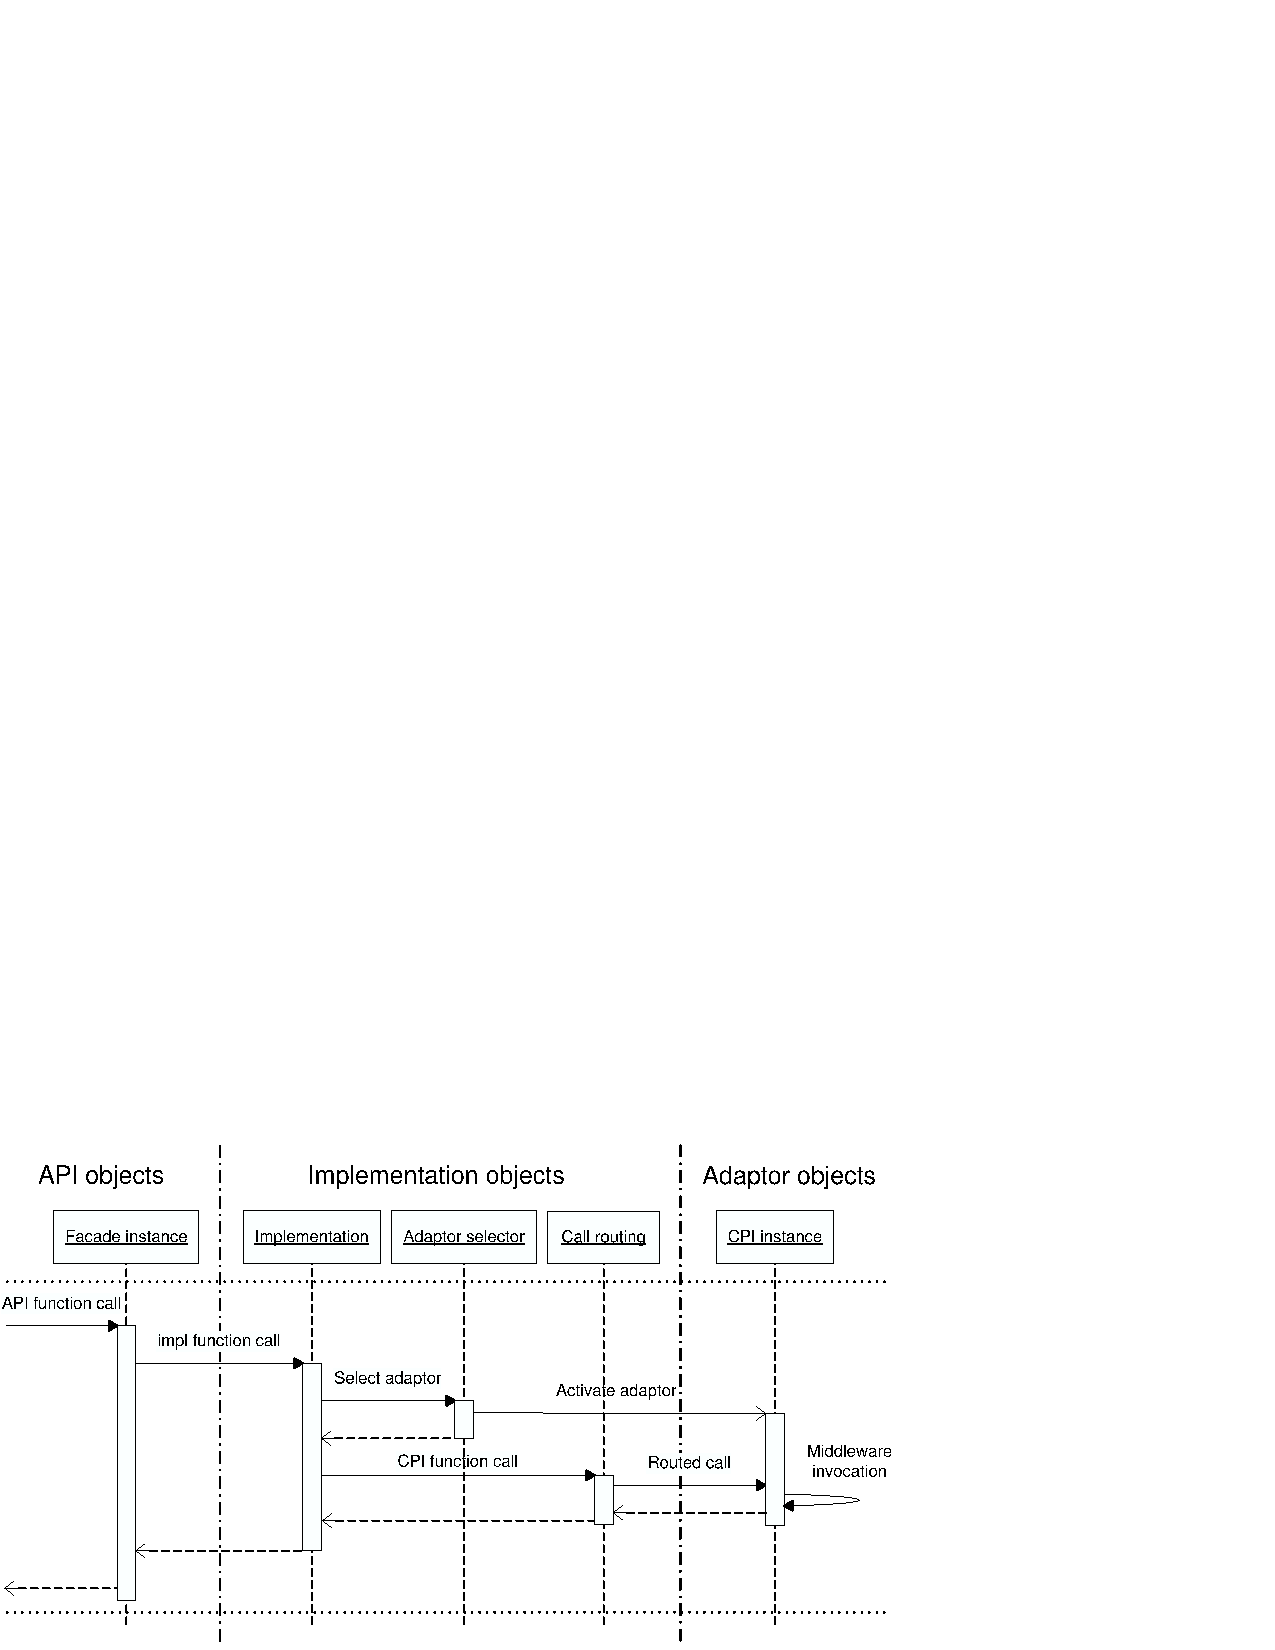
\includegraphics[width=0.45\textwidth]{../diagrams/object_lifetime_functioncall}
\caption{\label{fig:object_functioncall} API function call: Diagram
  illustrating the execution sequence through the different object
  instances during a call to any adaptor supplied function. The generic
  implementation of this call routing in the SAGA engine enables 
  interoperability because it provides the means of uniform selection of proper 
  middleware services based upon the specific application environment, 
  execution context, and user preferences.\upup}
\end{center}
\end{figure}




As stated above, in terms of interoperability the selection of
suitable adaptors at runtime is a central feature in our library
implementation (see figure~\ref{fig:object_functioncall}).  Conceptually 
this is a  simple mechanism: on loading, the adaptor components
register their \I{capabilities} in the adaptor registry.  If a method
is to be executed, the adaptor selector searches that registry for all
adaptors implementing that methods capability.  All suitable adaptors
are then ordered (best/most suitable first), and are tried one-by-one,
until the method invocation succeeds. The adaptor selection again is
routed through SAGA engine components, generically implementing this
for any function to be routed to a CPI instance.

\subsection{Lessons Learnt}
\label{ssec:learntlessons}

This section will summarize the most important implementation properties
form the interoperability standpoint: 

\begin{shortlist}
\item \I{Uniformity over Programming Languages:} Our implementation
  follows the SAGA API specification closely. It is also designed to
  accommodate wrappers in other languages, to provide the same
  semantics, and similar look\,\&\,feel to other language bindings.  A
  Python wrapper for our library is in alpha status, and we plan to
  add similar thin wrappers to provide bindings to C, FORTRAN, Perl,
  and possibly others.
\item \I{Adaptability to Heterogeneous and Dynamic Environments:}
  Flexible adaptor selection, late binding, and fall back mechanisms
  allow for additional resilience against a dynamic and evolving run
  time environment.
\item \I{Modularity makes the Implementation Extensible:} The
  adaptor mechanism allows for easy extensions of the library, to
  provide additional middleware bindings.
\item \I{Portability and Scalability:} Our library implementation is
  in fact very portable, as we strictly adhere to the C++ standard and
  portable libraries.  In fact, we currently develop the library on
  Windows, Mac and Linux concurrently, so we are confident that we are
  able to cover the three major target platforms without any problems.
\end{shortlist}

%Heterogeneous distributed systems require portability. 

\section{Demonstrating Interoperability}\label{sec:app}

We will outline two applications that demonstrate the connection
between SAGA and ALI. In the first application, we show how a SAGA
based application exploits ALI in order to implement its
functionality; in the second example, we show how SAGA provides 
simple implementation of file access and management for different 
applications.

\subsection{Network Performance Aware Application:}
We being with a discussion of a network-centric application, that is
capable of acquiring application-specific network characteristic data,
determining {\it ideal} migration target based on network
characteristics and then to migrate itself across heterogeneous Grids
without any changes at the application level.  We demonstrate how it
can be used for gathering network characteristics for a Poisson
Equation solver; details of the
application %and measurement data gathered
can be found in Ref.~\cite{saga_escience2007}.

\begin{figure}
 \begin{center}
 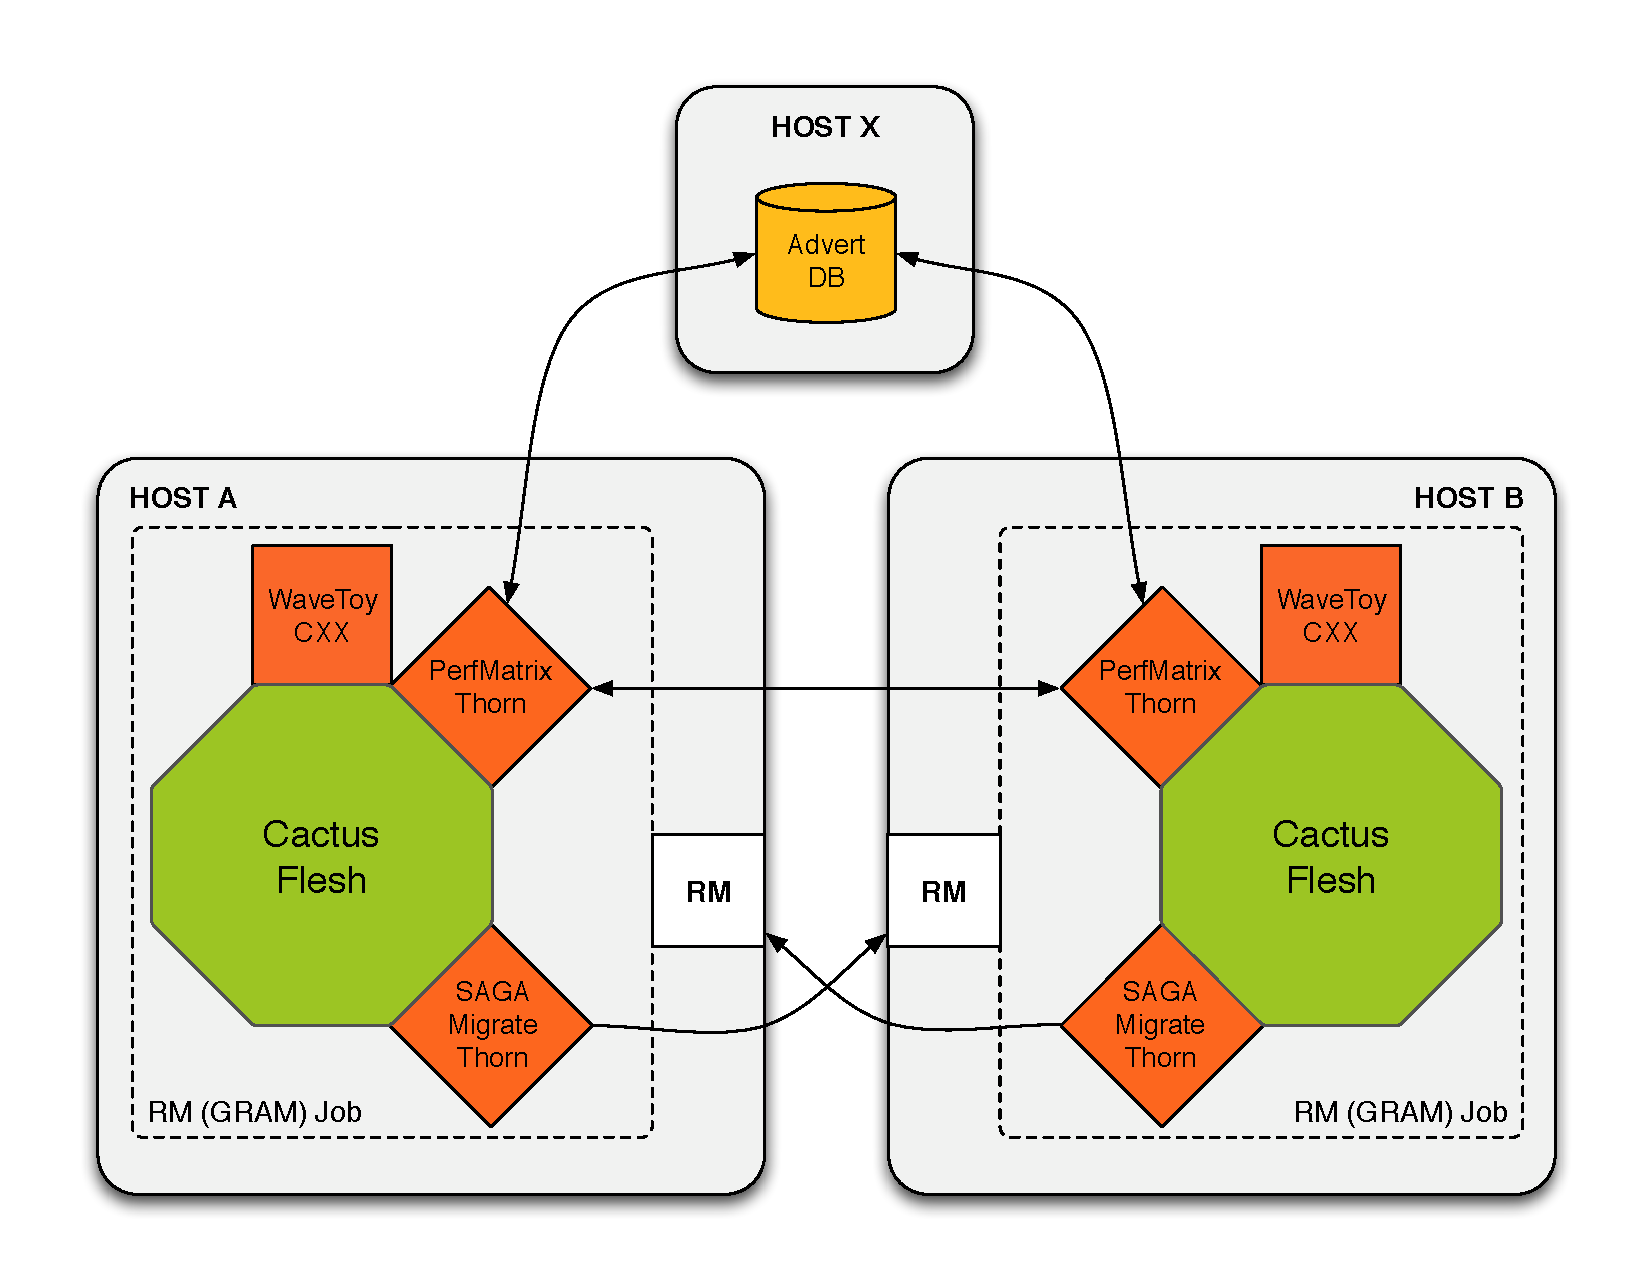
\includegraphics[scale=0.30]{../diagrams/figure_02}
\end{center}
\caption{The components of the application. The Cactus framework
  orchestrates the \textit{WaveToy} thorn as an example for a
  distributed calculation, the \textit{NetPerf} thorn for network
  performance measurement, and the \textit{SAGA Migration} thorn for
  replication and migration. The \textit{Advert DB} stores and
  archives the measurement results. Note that the application runs
  under the control of a \textit{Resource Manager (RM)} using SAGA's
  job management package.\upup}
 \label{fig:app_arch}
\end{figure}

The general architecture of the model application is based on the
programming abstraction provided by SAGA and the Cactus
framework~cite{X0}.  A set of thorns that provide specific
functionality are orchestrated by the Cactus flesh as depicted in
Fig.~\ref{fig:app_arch}.  With the SAGA functionality available it was
easy to implement Cactus thorns that can interact with remote resource
mangers (e.g. Globus GRAM2), copy, read, and write files from and to
remote locations (e.g.  Globus GridFTP), and access a remote
PostgreSQL based advert service as logging and storage facility. We
refer the reader to Ref.~\cite{saga_escience2007} for a detailed
discussion of the architecture, implementation and description of the
individual thorns; here we will discuss mainly the PerfMatrix thorn,
which takes care of the intrinsic network performance measurement and
persistent storage of the results.
\noindent{\it PerfMatrix Thorn:} The PerfMatrix algorithm uses a list
of computational resources which are potential migration targets for
the application. After starting up, the initial application spawns
itself onto all available hosts.  Once all jobs have been launched,
the original spawning application first establishes netperf~\cite{netperf_url}
connections with all the spawned applications; this is followed by the
spawned applications establishing netperf connections amongst each
other, following the scheme shown in Fig.~\ref{fig:algo}.  Job
spawning, control, and I/O redirection is done entirely using SAGA's
job management package.  Once a netperf process returns a throughput
result, the PerfMatrix thorn uses the SAGA advert-service package to
announce the result to a central database. After all netperf processes
have finished and published their results, the database contains a
host-to-host throughput performance matrix along with a timestamp
which is available to other thorns as well as other applications.
\begin{figure}
\begin{center}
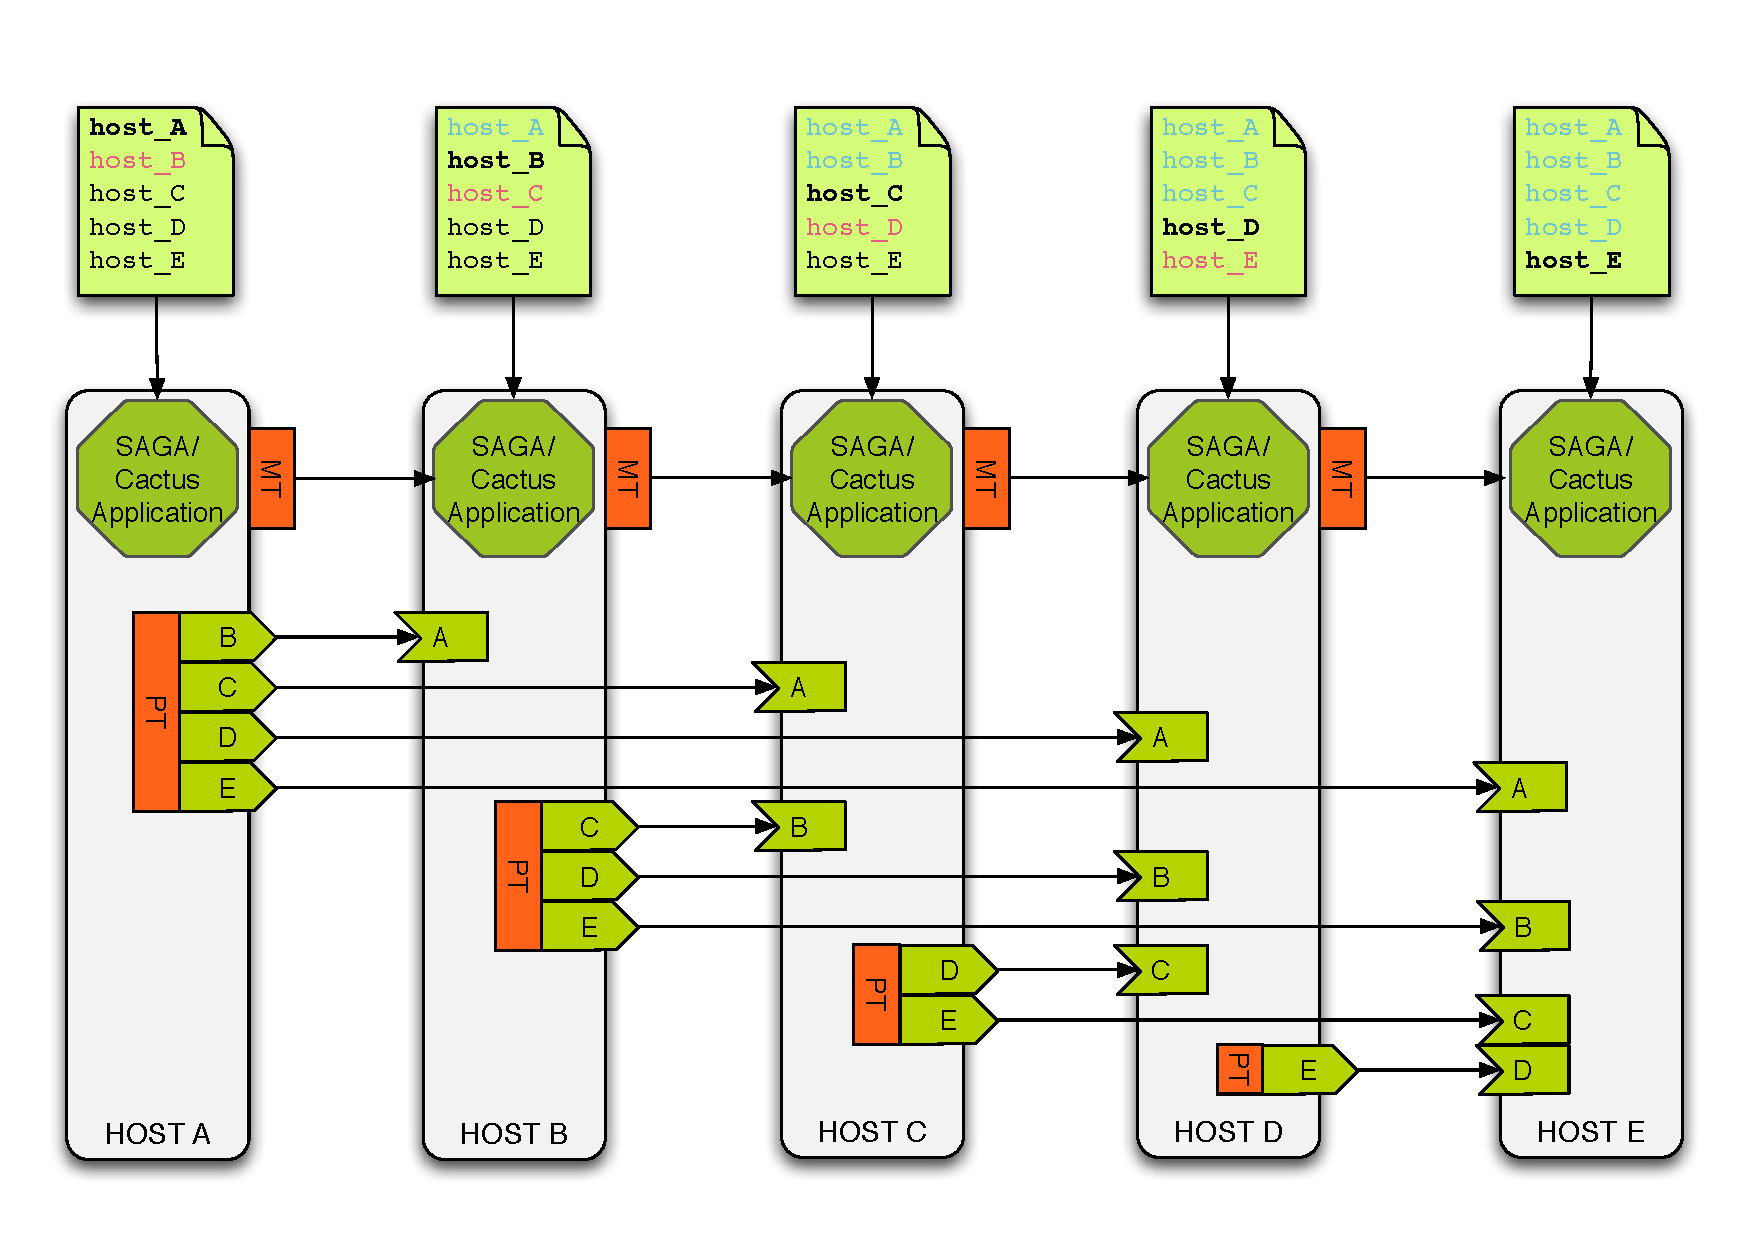
\includegraphics[scale=0.30]{../diagrams/figure_01}
\end{center}
\caption{The algorithm used by the PerfMatrix thorn. Based on a list
  of resources, the application spawns itself, launches Netperf
  endpoints and measures the throughput of all possible connections.\upup}
\label{fig:algo}
\end{figure}

\noindent{\it SAGAMigrate} The SAGAMigrate thorn is a Cactus thorn
written in C++ that uses SAGA functions (for example \T{file.copy} and
\T{job\_description.create\_job}) to perform a simulation migration.
SAGAMigrate copies a restart parameter file and the checkpoint file(s)
from one machine to another (for example using the SAGA Globus
adaptors).

An interesting feature of this application is {\it the ability to
  separate the computational logic from the distributed logic}. For
example, jobs on different resources, establish connections pairwise
and collect information which is published to an advert service
through SAGA's job-management package, whilst the PerfMatrix thorn
remains independent of the distributed aspects of the set of netperf
end-points.  This arises from using the correct abstractions (SAGA and
Cactus) and enables the application to be easily generalized to more
complex network performance requirement scenarios.  This application
can be deployed on any resource independent of the middleware stack.
All that is required is support for SAGA {\it adaptors} and the
corresponding client side middleware bindings. Thus beyond compiling
the application code on the other resources, there is no need for the
application to know about the details of the middleware or platform
details of the remote resources, whilst all along working across
distinct Grids!

\up
\subsection{Seamless Integration of Heterogeneous Grid Resources 
            using SAGA and FUSE}

\begin{figure}
\begin{center}
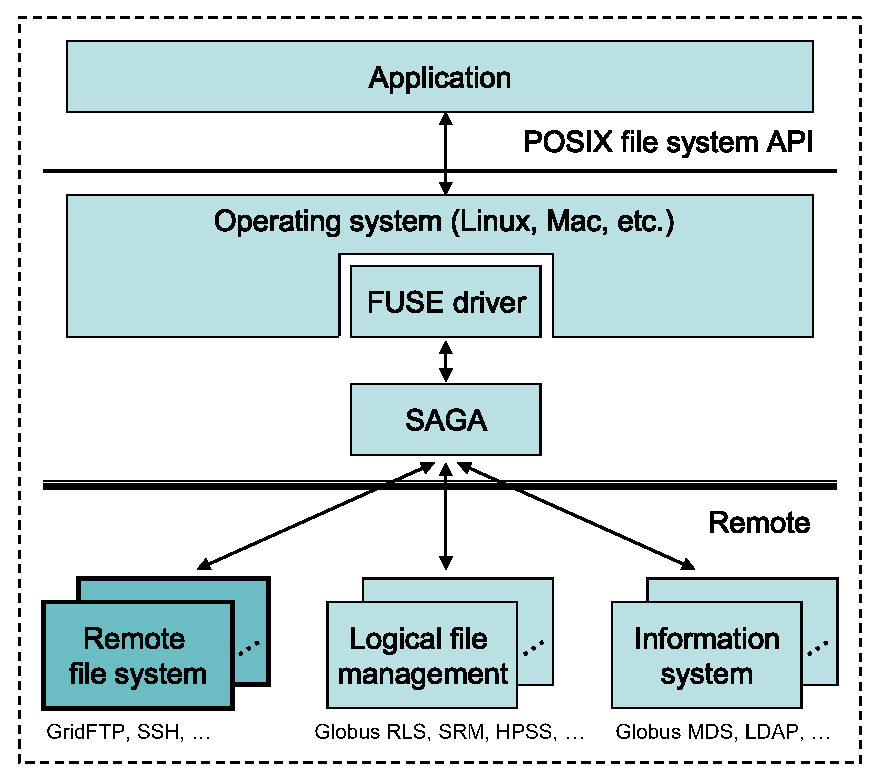
\includegraphics[scale=0.45]{../diagrams/FUSE_SAGA}
\end{center}
\caption{Any application can access remote files by using the POSIX filesystem
         API. The operating system dispatches these calls to the FUSE
         driver, which in turn uses SAGA to execute the required operation.\upup}
\label{fig:fuse_saga}
\end{figure}

% Another demonstration of SAGA for providing ALI, is the implementation
% of a filesystem driver for Linux and Mac.  

Another demonstration of how SAGA can enable seamless data management
and movement across different Grids, is the implementation of a
filesystem driver.  The filesystem driver is written using the FUSE
(Filesystem in UserSpace)~\cite{fuse_web} library and allows any
remote filesystem supported by a SAGA adaptor to be mounted onto a
local directory.  This driver uses SAGA to access remote filesystems
through different services, such as GridFTP or SSH.
Figure~\ref{fig:fuse_saga} shows the architecture of this application.
Other filesystem types can be seamlessly added just by writing
appropriate SAGA adaptors. Since the filesystem drivers are integrated
into the operating system, it makes the remote files available to any
application running on this system.

%No change to the applications itself is needed.

% \section{Discussion of the other aspects of this Work} \label{sec:discuss}
% % \textcolor{blue}{Jha, Ole}}

% The following are ensuing advantages of proper programming
% abstractions, but are not the primary focus of this current paper;
% these issues are dealt with at greater length in Ref.~\cite{saga_escience07}.

% \noindent {\it Demonstrate the usefulness of SAGA for Grid application
%   development:} SAGA provides a high-level programming interface to
% Grid functionality, and thus presents arguably, for the first time
% ever, the ability to develop complete and sophisticated applications
% using simple Grid function calls.  This paper demonstrates the utility
% of SAGA for creating applications that can perform across dynamic and
% heterogenous infrastructure.

% \noindent {\it Utilize the advantages of proper programming
%   abstractions: Integrate SAGA and Cactus}


\section{Conclusion} % \textcolor{blue}{Jha, All}}


% We also discussed how the deployment of this model application across
% two distinct Grids was trivial as it only required the deployment of
% of the appropriate SAGA adaptors.  

As efforts by the GIN community-group and other application-specific
groups have shown, interoperation is a hard problem to solve and
interoperability even harder! In this paper we discuss how each level
of the SAGA landscape -- interface specification, the engine and
middleware specific adaptors - contributes to providing application
level interoperability.  There are many applications that need to use
federated Grids~\cite{clade06, gin_paper}, and utilizing SAGA to
develop the Grid functionality of these applications provides an
effective way to do so.

On the other hand, if the development and deployment of applications
across federated Grids is to be facilitated, support and development
for SAGA adaptors for different middleware needs to be forth-coming and
self-sustaining and will thus require explicit support, from both the
middleware developers and resource providers.  Although, it might be
debatable as to when exactly a critical mass of the community threw
their support behind MPI, but irrespective of the timing, it is clear
that the technical merits of MPI coupled with the fact that it was a
community standard played a great role in increasing the number of
applications developed using MPI and the number of vendors that were
willing to support it -- thus providing MPI-based applications the
ability to interoperate across different parallel platforms. As SAGA
becomes a standard~\cite{saga-uc, saga-req, saga-core} there will be
increased willingness on the part of middleware developers and
resource providers to provide these adaptors to the application
community.  Additionally, as the deployment of SAGA and required
adaptors becomes wider (pervasive) and deeper (greater functionality),
there is an increased incentive for application developers to use
SAGA.

Making the global infrastructure a reality, critically depends upon
the availability of computational infrastructure that provides
resources that can be seamlessly used; developing both applications
and tools using SAGA is an effective mechanism for ensuring such
interoperability.% across different middleware distributions.

\section{Acknowledgements}

This work has been made possible thanks to the internal resources of
the Center for Computation \& Technology (CCT) at Louisiana State
University.  Important funding for SAGA specification and development
has been provided by the UK EPSRC grant number GR/D0766171/1 (via
OMII).  We would like to acknowledge the support of the OGF SAGA
Research Group for their work towards developing the SAGA
specification. We thank Yaakoub El Khamra and others from the Cactus
team; we also thank Chris Miceli - an undergraduate student in the
SAGA group for working on SAGA validation tests and the SAGA-FUSE
project. Finally, SJ acknowledges the e-Science Institute, Edinburgh
for supporting the theme, ``Distributed Programming Abstractions''.

\bibliographystyle{IEEEtran}
\bibliography{saga_gin}

\end{document}


% \amnote{MPI is a perfect example IMHO - compiling an MPI code with
% MPICH-G instead of some local MPI gives ALI.}

% \jhanote{In a way the important difference between ALI and SLI is
%  vertical versus hortizontal}

% Is it OK to say that SLI is a necessary condition, but not sufficient
% condition for ALI?

% Can we say find applications that are indpendent of SLI but require
% ALI?  (yes, any master-client programming model application does),
